\documentclass[11pt]{article}
\usepackage{../../cs70}
\usepackage{color}
\newif\ifsolutions
\solutionstrue
\solutionsfalse %flag for solutions

\def\title{Discussion 11A}
\begin{document}
\maketitle


\begin{enumerate}


\item {\bf Random Band} 

  In a group of ten people, seven can play the keyboard, five can play the guitar, four can play the violin, four can play the keyboard and the guitar, three can play the keyboard and the violin, two can play the guitar and the violin, and one person can play all three instruments. 

	\begin{enumerate}
	\item Suppose a person is picked uniformly at random from the group. Draw a Venn Diagram and use it to calculate the probability that this person can play at least one instrument. 
	\vspace{40mm}

	\ifsolutions{\color{blue}{
	\vspace{-40mm}
	{\bf Solutions:}
	\begin{figure}[h!]
	\center
	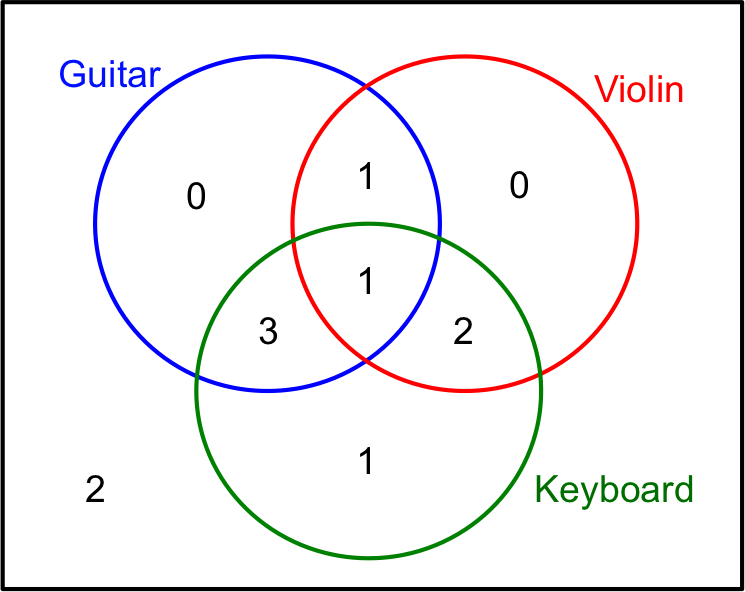
\includegraphics[width=0.4\textwidth]{band.png}
	\end{figure}

	Therefore the probability a randomly chosen person can play at least one instrument is $\frac{8}{10} = \frac{4}{5}$.
    	}} \fi

	\item Let $P(K)$ be the probability a randomly chosen person plays the keyboard, $P(G)$ be the probability a randomly chosen person plays the guitar, and $P(V)$ be the probability that a randomly chosen person plays the violin. Use the Inclusion-Exclusion principle to calculate the same probability as in part (a).
	\vspace{30mm}

	\ifsolutions{\color{blue}{
	\vspace{-30mm}
	{\bf Solutions:}
	\[ P(K) + P(G) + P(V) - P(K,G) - P(K,V) - P(G,V) + P(K,G,V) \]
	\[ = \frac{7}{10} + \frac{5}{10} + \frac{4}{10} - \frac{4}{10} - \frac{3}{10}  - \frac{2}{10} + \frac{1}{10} = \frac{8}{10} = \frac{4}{5} \]  
    	}} \fi

    	\end{enumerate}


\item {\bf Boy or Girl Paradox}
	\begin{enumerate}
	\item Mr. Smith has two children, at least one of whom is a boy. What is the probability that both children are boys?
	\vspace{50mm}

	\ifsolutions{\color{blue}{
	\vspace{-50mm}
	{\bf Solutions:} Let $B_1$ be the event that the first child is a boy, and $B_2$ be the event that the second child is a boy. We are asked to find 		$Pr[(B_1 \cap B_2) | (B_1 \cup B_2)]$:
	\begin{eqnarray*}
	Pr[(B_1 \cap B_2) | (B_1 \cup B_2)] &=& \frac{Pr[(B_1 \cap B_2) \cap (B_1 \cup B_2)]}{Pr[B_1 \cup B_2]}\\
	&=& \frac{Pr[B_1 \cap B_2]}{Pr[B_1] + Pr[B_2] - Pr[B_1 \cap B_2]}\\
	&=& \frac{\frac{1}{2} \cdot \frac{1}{2}}{\frac{1}{2} + \frac{1}{2} - \frac{1}{4}} = \frac{\frac{1}{4}}{\frac{3}{4}}\\
	&=& \frac{1}{3}
	\end{eqnarray*}

	\textbf{Note:} It is tempting to think that because the children's genders are independent, the probability of the second child being a boy given that the first is a boy is simply $\frac{1}{2}$. While this is true, when we write it out in terms of events, we can see that this is not the quantity that we want (that is, $Pr[B_2 | B_1]$, which is not what we found above).

	}} \fi

	\item Mr. Smith has two children, one of whom is a boy born on a Tuesday. What is the probability that both children are boys?
	\vspace{50mm}

	\ifsolutions{\color{blue}{
	\vspace{-50mm}
	{\bf Solutions:} Consider a 14 by 14 table listing out all possible combinations of each child's gender and birth day-of-week.
	We know that at least one boy is born on a Tuesday, so we are only concerned with one row and one column of the table (the boy-born-on-Tuesday row and column).
	There are $14+14-1=27$ cells in this part of the table. In $13$ of these $27$ cells, there are two boys.
	Therefore, Mr. Smith has a $\frac{13}{27}$ probability of having two boys, given that one of his two children is a boy born on Tuesday.

Alternatively, consider working with probabilities. We define the following events:
\begin{eqnarray*}
A &=& 1^{st} \text{ child is a boy}\\
B &=& 1^{st} \text{child was born on Tuesday}\\
C &=& 2^{nd} \text{ child is a boy}\\
D &=& 2^{nd} \text{child was born on Tuesday}\\
E &=& \text{at least one child is a boy born on Tuesday}
\end{eqnarray*}
From this, we can see that we are interested in
\begin{eqnarray*}
Pr[(A \cap C) | E] &=& \frac{Pr[(A \cap C) \cap E]}{Pr[E]}\\
&=& \frac{Pr[E | (A \cap C)] Pr[A \cap C]}{Pr[E]}
\end{eqnarray*}
To calculate $Pr[E]$:
\begin{eqnarray*}
Pr[E] &=& Pr[(A \cap B) \cup (C \cap D)]\\
&=& Pr[A \cap B] + Pr[C \cap D] - Pr[(A \cap B) \cap (C \cap D)]\\
&=& Pr[A]Pr[B] + Pr[C]Pr[D] - Pr[A \cap B]Pr[C \cap D]\\
&=& \frac{1}{2} \cdot \frac{1}{7} + \frac{1}{2} \cdot \frac{1}{7} - (\frac{1}{2} \cdot \frac{1}{7})(\frac{1}{2} \cdot \frac{1}{7})\\
&=& \frac{27}{196}
\end{eqnarray*}
Plugging into our expression from before,
\begin{eqnarray*}
Pr[(A \cap C) | E] &=& \frac{Pr[(A \cap C) \cap E]}{Pr[E]}\\
&=& \frac{(\frac{1}{7} + \frac{1}{7} - \frac{1}{49})\frac{1}{2} \cdot \frac{1}{2}}{\frac{27}{196}} = \frac{\frac{13}{196}}{\frac{27}{196}}\\
&=& \frac{13}{27}
\end{eqnarray*}
	
\textbf{Note:} This result is very different from our intuition! Moral of the story? You can't always trust your intuition to be correct! Always define events and work through the probabilities first!

}} \fi

\end{enumerate}

\ifsolutions{\color{blue}{
Note: For both parts, assume that the probability of a boy or girl being born is the same, a child is equally likely to be born on any day of the week, and the genders of all children are independent of each other and independent of the day of the week.

}} \fi
   
\item Prove that in every probability space, if $A$ and $B$ are independent events, then $\overline{A}$ (not $A$) and $\overline{B}$ (not $B$) are also independent. {\em Hint: use Inclusion-Exclusion.}

\ifsolutions{\color{blue}{
	{\bf Solutions:}

Note: The most general version of this theorem states that if $A_1,\ldots,A_n$ are a fully independent collection of events, then you can take any subcollection and replace them by their complements, and it will still be fully independent. Intuitively, this should not come as a surprise, and you're free to use this fact throughout the course. It can be proven using the inclusion-exclusion principle, though we do not ask you to do that.

\textbf{Proof:} We will use a direct proof. Assume that $A$ and $B$ are independent events. If either $\text{Pr}[A]$ or $\text{Pr}[B]$ are either 1 or 0, then $A$ and $B$ are trivially independent. In the nontrivial case, to show that $\overline{A}$ and $\overline{B}$ are independent, it will suffice to show that $\overline{A}$ and $B$ are independent (because we can then use the same process to show that $\overline{A}$ and $\overline{B}$ are independent).
By total probability, we have $\text{Pr}[B]=\text{Pr}[B|A]\text{Pr}[A]+\text{Pr}[B|\overline{A}]\text{Pr}[\overline{A}]=\text{Pr}[B]\text{Pr}[A]+\text{Pr}[B|\overline{A}]\text{Pr}[\overline{A}]$, where $\text{Pr}[B|A]=\text{Pr}[B]$ follows from the independence of $A$ and $B$.
Subtracting $\text{Pr}[B]\text{Pr}[A]$, we get $\text{Pr}[B](1-\text{Pr}[A])=\text{Pr}[B|\overline{A}]\text{Pr}[\overline{A}]$. Since $1-\text{Pr}[A]=\text{Pr}[\overline{A}]$, we can divide them out and get $\text{Pr}[B]=\text{Pr}[B|\overline{A}]$. This shows that $\overline{A}$ and $B$ are independent, which shows that $\overline{A}$ and $\overline{B}$ are independent. $\blacksquare$


Alternatively, consider another approach. We will use a direct proof. Assume that $A$ and $B$ are independent events. This means that $\text{Pr}[A\cap B]=\text{Pr}[A]\text{Pr}[B]$.
Important to note is that $\overline{A}\cup\overline{B}$ is the complement of $A\cap B$, so $\text{Pr}[\overline{A}\cup\overline{B}]=1-\text{Pr}[A\cap B]$.
Let's then start with the inclusion-exclusion principle, $\text{Pr}[\overline{A}\cup\overline{B}]=\text{Pr}[\overline{A}]+\text{Pr}[\overline{B}]-\text{Pr}[\overline{A}\cap\overline{B}]$ and put it into the form $\text{Pr}[\overline{A}\cap\overline{B}]=\text{Pr}[\overline{A}]+\text{Pr}[\overline{B}]-\text{Pr}[\overline{A}\cup\overline{B}]$.
\begin{eqnarray*}
\text{Pr}[\overline{A}\cap\overline{B}]&=&\text{Pr}[\overline{A}]+\text{Pr}[\overline{B}]-\text{Pr}[\overline{A}\cup\overline{B}]\\
                                       &=&\text{Pr}[\overline{A}]+\text{Pr}[\overline{B}]-(1-\text{Pr}[A\cap B])\\
                                       &=&\text{Pr}[\overline{A}]+\text{Pr}[\overline{B}]-(1-\text{Pr}[A]\text{Pr}[B])\\
                                       &=&\text{Pr}[\overline{A}]+\text{Pr}[\overline{B}]-(1-(1-\text{Pr}[\overline{A}])(1-\text{Pr}[\overline{B}]))\\
                                       &=&\text{Pr}[\overline{A}]+\text{Pr}[\overline{B}]-(1-1+\text{Pr}[\overline{A}]+\text{Pr}[\overline{B}]-\text{Pr}[\overline{A}]\text{Pr}[\overline{B}])\\
                                       &=&\text{Pr}[\overline{A}]+\text{Pr}[\overline{B}]-\text{Pr}[\overline{A}]-\text{Pr}[\overline{B}]+\text{Pr}[\overline{A}]\text{Pr}[\overline{B}]\\
\text{Pr}[\overline{A}\cap\overline{B}]&=&\text{Pr}[\overline{A}]\text{Pr}[\overline{B}] \text{ }\blacksquare
\end{eqnarray*}

}} \fi

\end{enumerate}

\end{document}
